This chapter offers an overview of the different implementation steps to develop the project.

\section{System Architecture Overview}

Follow low-level implementation detail of the different stages of the pipeline.\\

Include code snippets for individual sections.

% \begin{figure}[h] 
% \centerline{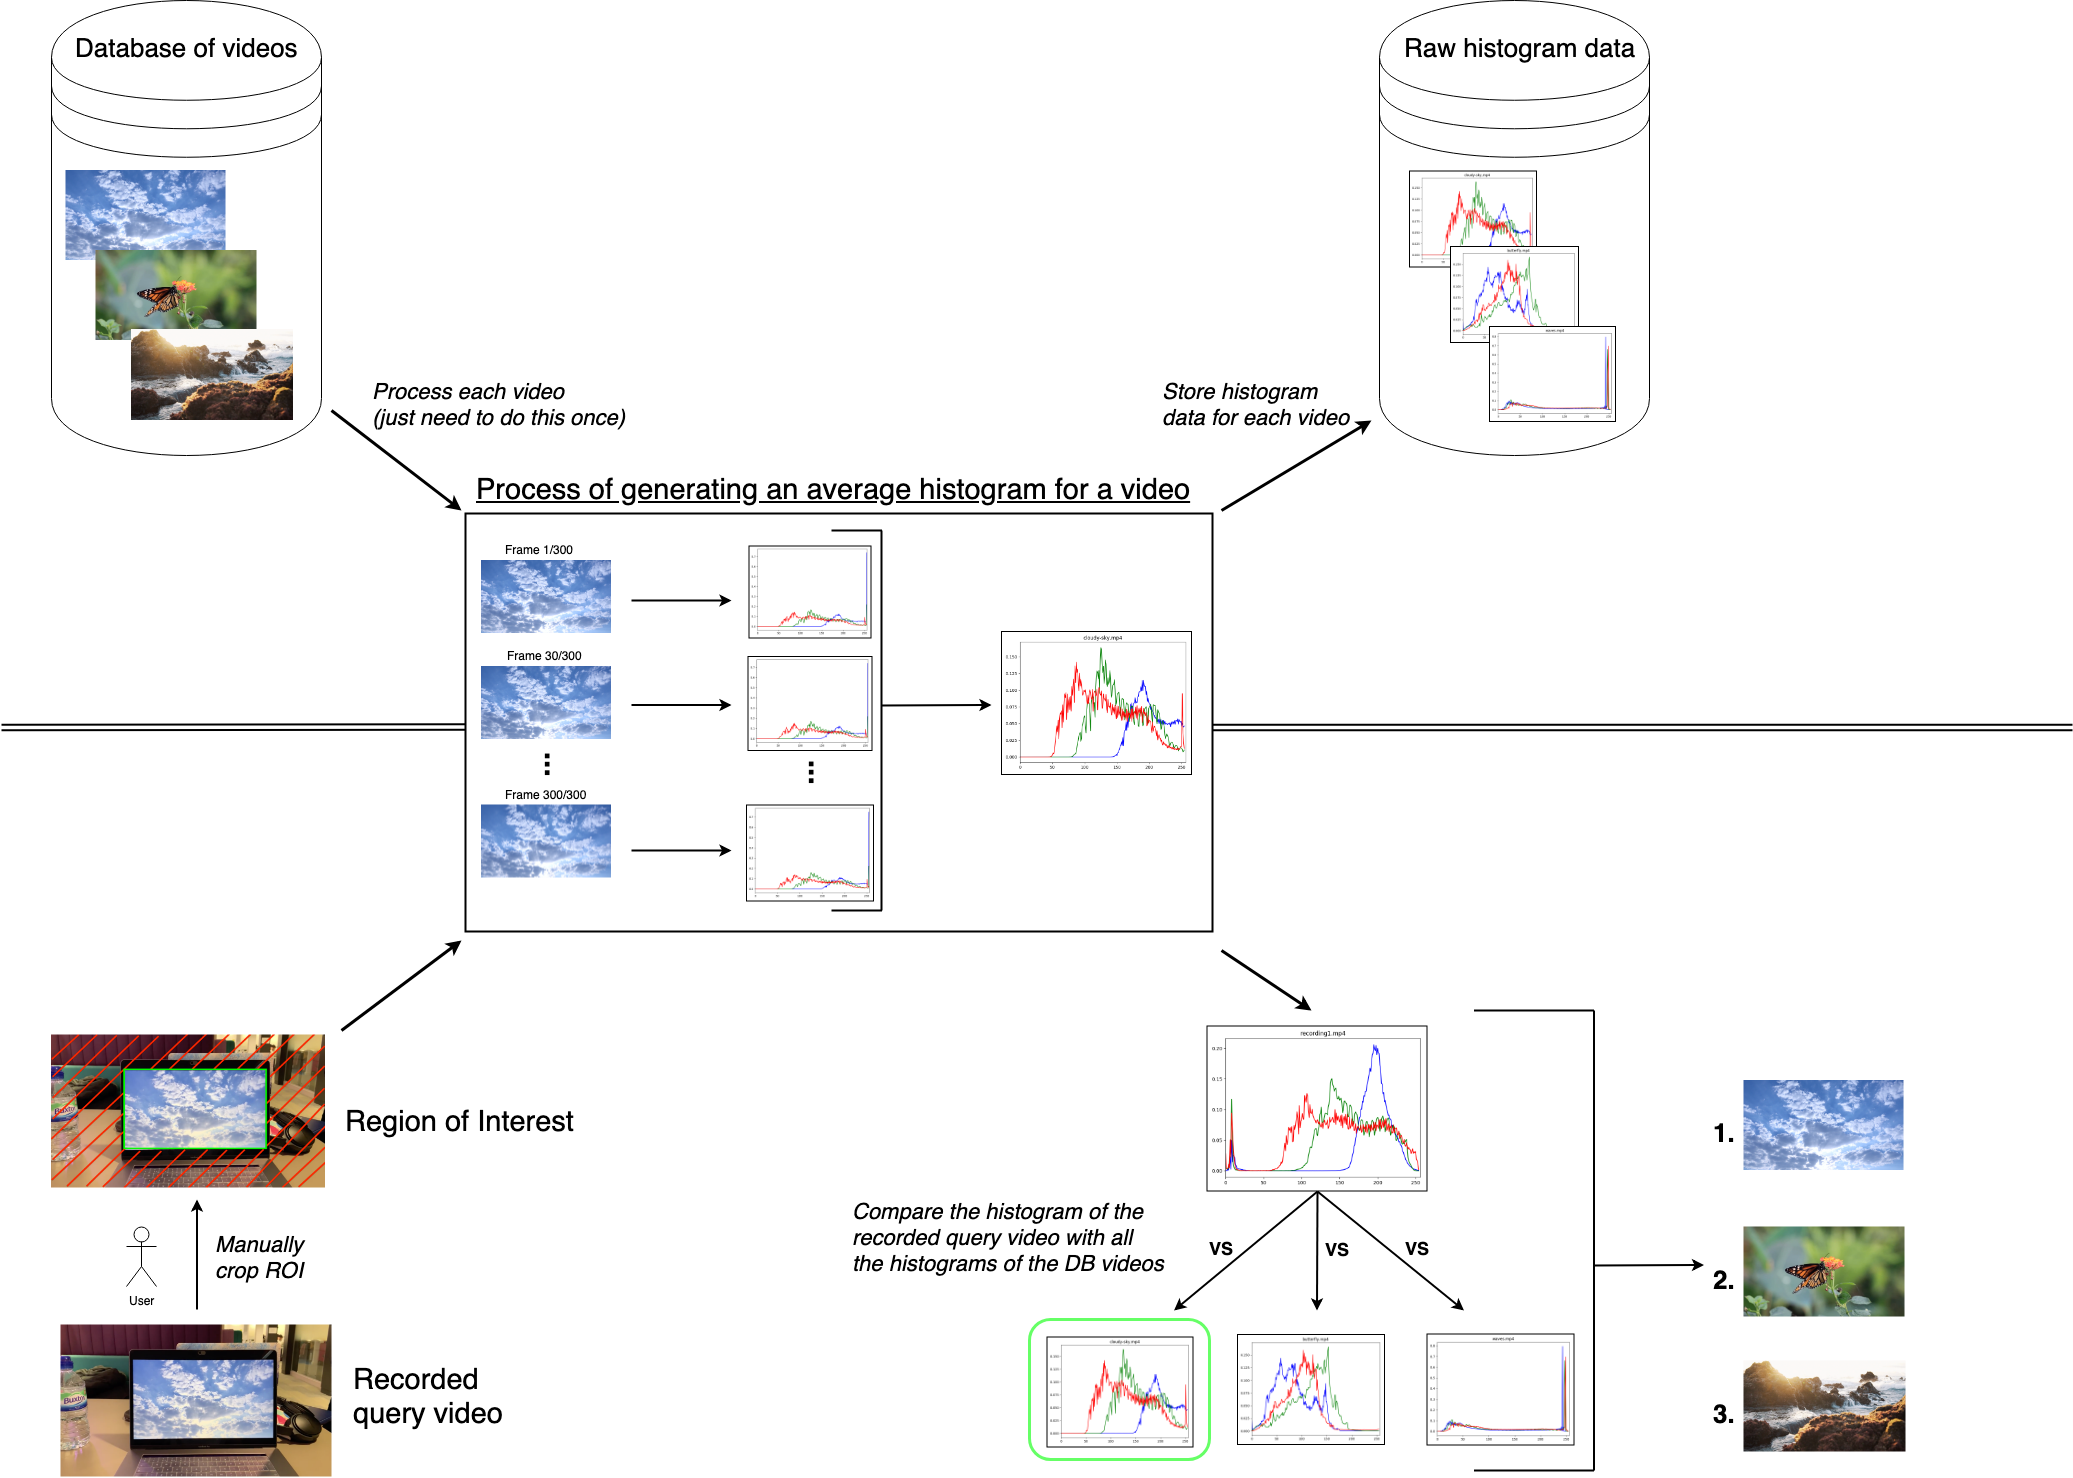
\includegraphics[width=\textwidth]{figures/implementation/CBVR-flowchart.png}}
% \caption{\label{fig:CBVR flowchart}Flowchart.}
% \end{figure}

\section{Offline Colour-Based Feature Extraction}

This section details the different steps that go towards generating histograms and creating the compact signature used to represent each video.

\subsection{Histogram Generation}

1 frame every 30 frames retrieved

\subsubsection{RGB Histogram Generation}

The first type of histogram that is generated is the RGB histogram. As described in \ref{sec:color-based-features}, an RGB histogram represents the colour distribution of the pixels in a frame for three different channels: red, blue and green. To calculate an RGB histogram, OpenCV's \textit{calcHist()} method is used, as shown in Listing \ref{listing:generate_rgb_hist}. 

\begin{listing}[h]
\inputminted
[
baselinestretch=0.9,
bgcolor=LightGray,
fontsize=\footnotesize,
linenos,
breaklines,
]
{python}{code-listings/generate_rgb_hist.py}
\caption{Single RGB histogram generation}
\label{listing:generate_rgb_hist}
\end{listing}

\begin{figure}[h] 
\centerline{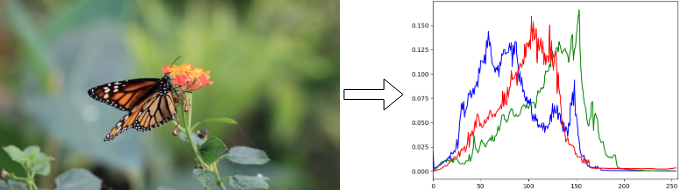
\includegraphics[width=\textwidth]{figures/implementation/rgb_histogram_generation.png}}
\caption{\label{fig:implementation-rgb_histogram_generation}Example of the three generated RGB histogram channels.}
\end{figure}

\subsubsection{Greyscale Histogram Generation}

A greyscale histogram is generated for each database video. 

\subsubsection{HSV Histogram Generation}

An HSV histogram is generated for each database video. 

\subsubsection{Creating Compact Video Signature}

averaging histogram
normalising
writing to human-readable txt file

\section{Online Retrieval}

query video, identical features extracted

\subsection{Query Video Pre-processing}

\subsubsection{Video Stabilisation}

video stabilised

\subsubsection{Region of Interest Selection}

roi selection

\subsection{Similarity Measurements}

distance measurements to find nearest neighbour between query histograms and each database video histogram:

\begin{itemize}
    \item correlation
    \item intersection
    \item chi-square
    \item alternative chi-square
    \item bhattacharyya
    \item kullback leibler divergence
    \item wassertein distance (Earth's Mover Distance)
    \item energy distance
\end{itemize}

combining results from all 3 methods with weight between different histogram methods to give more importance to HSV, GRB and less importance to grey scale: 1-5-10

\section{Database Pre-Processing}

\begin{itemize}
    \item shot boundary detection for long videos, allowing the entire movie to be represented with a few thousand frames
    \item current: one frame every second for short videos
\end{itemize}

\section{Output-Related}

\begin{itemize}
    \item opencv box drawing to select Region of Interest
    \item matplot lib histogram plotting (with an option to show each generated histogram or to hide them)
    \item tables to show scores for each type of histogram and each distance
    \item exporting results to CSV for further analysis
    \item spinners to show calculations are being done when training the system or stabilising videos 
    \item argument parsing
    \item final output to clearly show if result if right/wrong, including a frame of the original query video, a frame of the match found, along with the runtime and tha accuracy
\end{itemize}

\section{Testing}

\begin{itemize}
    \item Unit Testing
        \begin{itemize}
            \item grey scale / RGB / HSV histogram generation
            \item histogram saving to file
            \item histogram normalisation
            \item ROI selection
            \item individual histogram matching, test each metric
        \end{itemize}
    \item Integration Testing
        \begin{itemize}
            \item test the entire pipeline (with a few videos as the database, make sure the correct match is found)
        \end{itemize}
    \item Include some code snippets
    \item Include test suite results
\end{itemize}